\section{Results}

Using linear regression for the prediction of DTE for each driver along the circuit, we demonstrated that this approach can outperform the vehicles' own DTE estimation models, as seen in Figure \ref{fig:dte}.

\begin{figure}[!htb]
\centering
    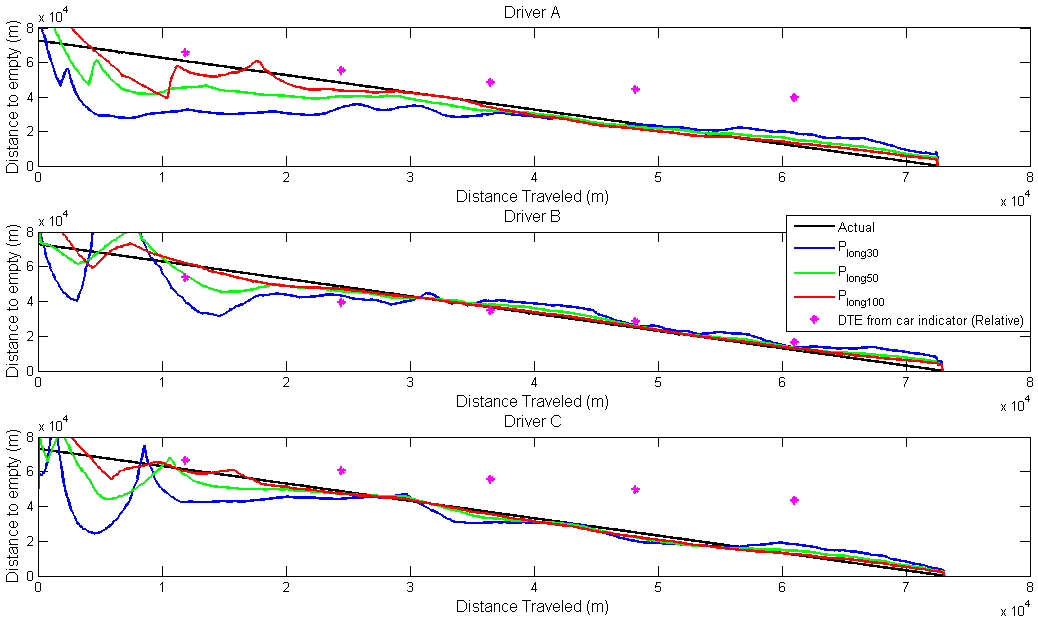
\includegraphics[width=0.5\textwidth]{figs/acmdte}
\caption{\(DTE\) estimated with different-sized terms of fuel intensity (\(p_{long}\)). Red dots are estimates given by in-vehicle displays.}
 \label{fig:dte}
\end{figure}

We then applied the extended modeling methodology to predict fuel consumption for each driver along each run along each route, using the data from them along other routes and other drivers along all routes. The resulting matrix of estimations, and their difference from actual consumption data, is shown in Table 1.

\begin{table}
\label{tab:est}
  \centering
  \begin{tabular}{|c|c|c|c|}
\hline
    Route & Driver A & Driver B & Driver C \\
\hline
\multirow{2}{*}{1} & 1.71 (10.0\%) & 1.23 (17.5\%) & 1.77 (18.8\%)\\
& 1.70 (12.1\%) & 1.18 (19.4\%) & 1.84 (18.6\%)\\
\hline
\multirow{2}{*}{2} & 0.88 (9.6\%) & 0.61 (10.9\%) & 0.81 (22.5\%)
\\
& 0.88 (14.6\%) & 0.59 (22.1\%) & 0.75 (30.7\%)
\\
\hline
\multirow{2}{*}{3} & 0.67 (10.2\%) & 0.57 (7.8\%) & 0.73 (8.7\%)
\\
& 0.65 (4.8\%) & 0.40 (23.2\%) & 0.73 (20.8\%)
\\
\hline
  \end{tabular}
  \caption{Estimation of fuel consumption in litres for each run of each route by each driver, with error in parentheses}
\end{table}
